\documentclass[class=minimal,border=2pt]{standalone}

\usepackage{tikz}
\usetikzlibrary{shapes,arrows}
\usepackage{verbatim}
\usepackage{pgfplots, pgfplotstable}

\begin{document}
	
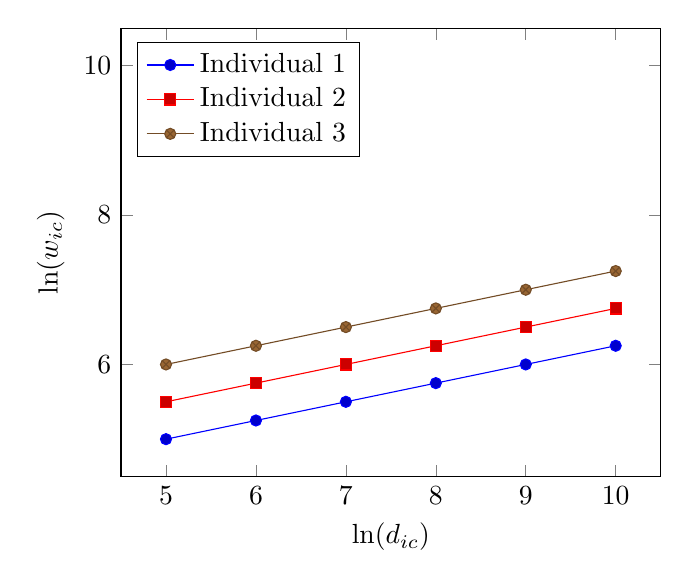
\begin{tikzpicture}
  \begin{axis}[
    xlabel = $\ln(d_{ic})$,
    ylabel = $\ln(w_{ic})$,
    legend pos = north west,
    ymin = 4.5,
    ymax = 10.5
    ]
    \addplot coordinates {
      (5, 5)
      (6, 5.25)
      (7, 5.5)
      (8, 5.75)
      (9, 6)
      (10, 6.25)
    };
    \addlegendentry{Individual 1}
    \addplot coordinates {
      (5, 5.5)
      (6, 5.75)
      (7, 6)
      (8, 6.25)
      (9, 6.5)
      (10, 6.75)
    };
    \addlegendentry{Individual 2}
    \addplot coordinates {
      (5, 6)
      (6, 6.25)
      (7, 6.5)
      (8, 6.75)
      (9, 7)
      (10, 7.25)
    };
    \addlegendentry{Individual 3}
  \end{axis}
\end{tikzpicture}
\end{document}